\documentclass{llncs}
\usepackage{graphics}
\usepackage[dvips]{epsfig}
\usepackage[latin1]{inputenc}
\usepackage{color}
\usepackage{longtable}
%\usepackage{multirow}
\usepackage[dvips]{graphicx} 
%\usepackage{amsmath}
\usepackage{textcomp}
\usepackage{url}
\usepackage{algpseudocode}

\newcommand{\tab}{\hspace{20mm}}

\setlength{\textfloatsep}{8pt plus 2pt minus 2pt}
\setlength{\intextsep}{8pt plus 2pt minus 2pt}

%#\def\BibTeX{{\rm B\kern-.05em{\sc i\kern-.025em b}\kern-.08em
%#    T\kern-.1667em\lower.7ex\hbox{E}\kern-.125emX}}

%\hyphenation{}


\begin{document}
\section{Fitness studied}
In our previous works, we evaluated a single bot of the population versus always the same bot (our reference-bot). For fitness function, the bot was evaluated several times (in different maps). The fitness function was defined depending of the result of the battle (if the bot win all his battles or lose in someone) and the numbers of turns needed for end the game. For two bots of the population (A and B) the fitness is defined like:

\begin{figure}
\begin{algorithmic}
\State{$A,B\in Population $}
\If {A WINs always}
    \If{B LOSEs some battle}
    	\State A is better than B
    \ElsIf{A take less turns than B}
    	\State A is better than B
    \Else
    	\State B is better than A
    \EndIf
\Else
     \If{B WINs always}
    	\State B is better than A
    \ElsIf{A take less turns than B}
    	\State B is better than A
    \Else
    	\State A is better than B
    \EndIf
\EndIf
\end{algorithmic}
\caption{Fitness used in battles of 2 bots}
\label{fig:fitness_clasico}
\end{figure}

This fitness works well for battles between two bots, and our first fitness proposed is an natural evolution of this fitness for 4 bots battles.

%However it'snt prepared for battles between 4 bots. For example, 2 bots that in their battleds finish in third place, it's best the one that take more turns or the other? The answer to this question, it's that depends of the other bots. Of course, all the fitness 

\subsection{Fitness based in Position-turns}

This fitness it's an natural evolution of the previous fitness, applied to 4 bots battles. Again, the evaluations are in several maps. In this case, we studie the position (1th,2th,..) of the bot in the 4-battle and the number of turns. For a bot that wins all the battles (it's 1th in all the battles) we call the sum of the numbers of turns {$ferocity$}, and in previous works we found that a bot that wins in less turns it's best that other that takes more turns (even if the both wins). In other case, the sum of turns is call {$sturdy$} and oposite to the {$ferocity$}, it's desirable a bot that take more turns in be defeated.

\begin{figure}
\begin{algorithmic}
\State{$A,B\in Population $}
\If {A WINs always}
    \If{B LOSEs some battle}
    	\State A is better than B
    \ElsIf{A take less turns than B}
    	\State A is better than B
    \Else
    	\State B is better than A
    \EndIf
\Else
     \If{B WINs always}
    	\State B is better than A
    \ElsIf{A take less turns than B}
    	\State B is better than A
    \Else
    	\State A is better than B
    \EndIf
\EndIf
\end{algorithmic}
\caption{Fitness used in battles of 2 bots}
\label{fig:fitness_clasico}
\end{figure}



The principal problem in the previous fitness, it's that there we are using two independents variables. In this case, we try to found a fitness that resume the goodness of our bot in a single number. %Describir ventajas de que un solo fitness, puede ser operado (sumado).

In this fitness, we are only interesting in the final result: position and turn. We aren't student how the bot reach it. In the nexts fitness, we use another metric to define the goodness of the bots. The percentage of the ships that in each turn belong to each player.

\begin{figure}
\begin{center}
  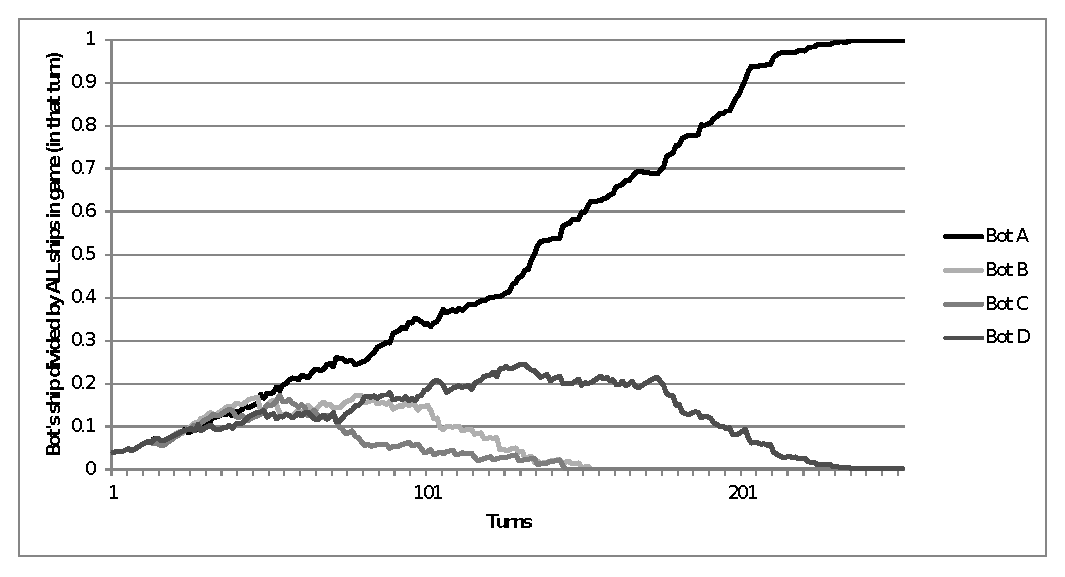
\epsfig{file=imagenes/nubecita.eps,width=9.2cm}
\end{center}
\caption{Representation of the number if ships of each bot in each turn} 
\label{figura:nubecita}
\end{figure}

\subsection{Fitness based in Slope}

For this fitness, we use the leats squares regression analysis for resume the cloud of points to a simple rect. The rect is represented as {$y = \alpha \times x + \beta $} where, {$\alpha$} and {$\beta$} are:

\begin{figure}
	\begin{equation}
		\alpha = \frac{\sum_{i=1}^{n}(X_{i} - \bar{X_{i}})(Y_{i} - \bar{Y_{i}})}{\sum_{i=1}^{n}(X_{i} - \bar{X_{i}})^{2}}
	\end{equation}
	\begin{equation}
		\beta = \bar{Y}-\alpha\bar{X}
	\end{equation}
\end{figure}

\begin{figure}
\begin{center}
  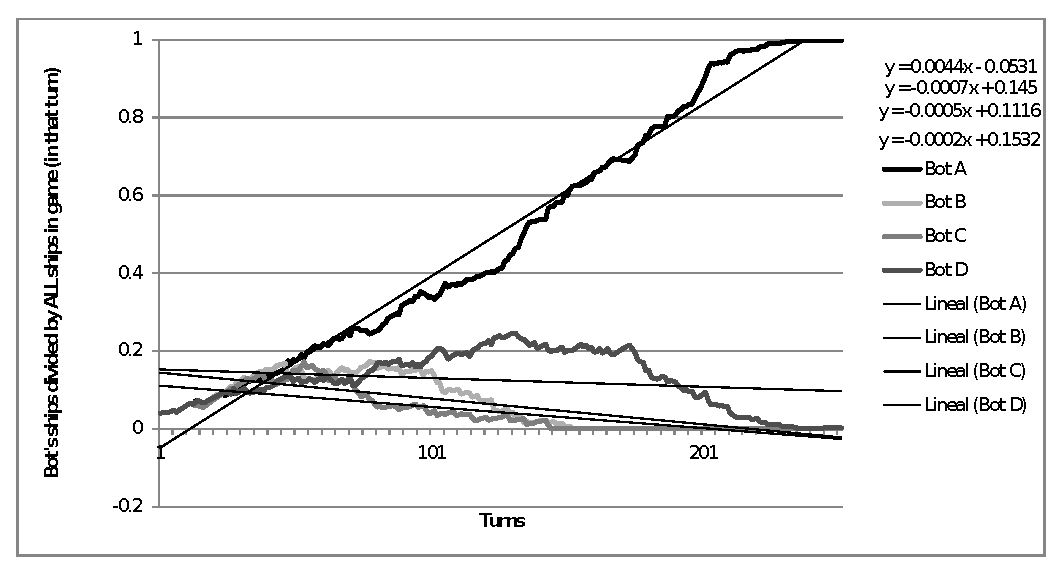
\epsfig{file=imagenes/nubecita_pendiente.eps,width=9.2cm}
\end{center}
\caption{Representation of the number if ships of each bot in each turn} 
\label{figura:nubecita}
\end{figure}



\subsection{Fitness bases in Integral-Area}

\label{sec:fitness}

\end{document}